\documentclass{article}
\usepackage{ben-basic}
\usepackage{multiaudience}
\SetNewAudience{fantasy}
\title{Effective Text Editing}
\begin{document}
\pdfbookmark[section]{Contents}{toc}
%\shorttoc{Contents}{1}
\tableofcontents
\clearpage

\showto{fantasy}{This only shows to the initiated.}

\section{Literature}
Test The most basic unit of textual information is not a letter, nor a word, but a sentence.  A letter or word are only supplemental by themselves, and if they hold any inherit meaning, it is only because they are implying a relative sentence.

A sentence is a standard grammatical formation of a statement, which (as it suggests) expresses some state.  Without state there is no activity, and without activity, no life.  Therefore, all proper writing is the conveyence of state colocation and transformation, within a given context.  The mastery of processing both sides of literature (e.g., reading, writing) is condusive to productivity as the requirements of complex engagements have either been resolved or a resolution thereof can be captured in text for posterity.

\section{Optimal Text-Editing}

For the business of applying text to paper, or to the electronic standard of the day, most start and end with rich text GUI editors like MS Word, or whatever comes with the typical email client.  Yet, even until this day, you will many in academia are still using Latex, a digital typesetting system, to compose highly sophisticated research papers.  What is the gap here?  While others say traditions and the pretty print achieved by Tex outputs, I say that the really difference is scaffolding.

Any sophisticated building project requires scaffolding in order to quickly navigate the building until the infrastructure is complete.  WYSIWYG editors by their very nature cannot do this.  A comment or discretionary text is anti-thetical to the original intent of editors like Word and Word Perfect; that is to maintain an editing view that looks as close to the final view as possible.

Why Vim fluency vs mouse clicking and standard control keys?

The following key commands are helpful and available on most GUI systems:
* CTRL-F (find)
* CTRL-C/X/V (copy, cut and paste)

Combined with mouse controls, is sufficient for quick, short, one-off documents; but any document that may require much rearrangement, and scaffolding, would be better served by vim key binding, which excels at moving around various text strings.

Shell program vs GUI IDE


% \subsection{Secondary-Reason}
A secondary reason to prefer document creation with tools such as Vim and Latex, over word processors like Microsoft Word, is simply reliability.  Among all applications that are highly productive, robust and ubiquitous, there archetype less "buggy" and more responsive than the simple text editor.  Other applications, mostly GUIs, in attempt to try and model the world to make the platform more intuitive causes every keystroke to behave as a resounding gong in a crowded theatre, evoking many different agents to check, sometimes change and re-check every other element related to the document.  This can grind the performance of a Word processor, and its host to a fault; facilitating editing errors due to an irresponsiveness to commands. 

\section{Latex}
\subsection{Custom Styles}
To prevent the having to copy styles to each latex project on the same host, simply add the style to a texmf (i.e., Tex Metafont) directory, and register it by running the following commands:
mkdir -p ~/texmf/tex/latex
cp <your custom style> ~/texmf/tex/latex
texhash

%TODO credit https://www.ias.edu/math/computing/faq/local-latex-style-files

\section{Git}
\subsection{Authentication Method Ranking}
There are three main options for establishing authentication for write actions like a "push" with a Git.  My criteria for considering both security and productivity results in the following preference order: SSH, password access tokens, password client managers.  SSH is always my first choice, because it offers great convenience and high security standards with the use of the latest RSA public-key encryption.  Yet, some network environments may not allow SSH throughput, therefore "password access tokens" can be used against HTTPS with minimal effort.  As far as password manager clients, it nearly goes without saying that the cumbersome aspect of installing more software to config and set up is not compelling, although, it may offer better security of HTTPS if your current file system is secure.
\subsubsection{SSH}

\subsubsection{Password Access Tokens}

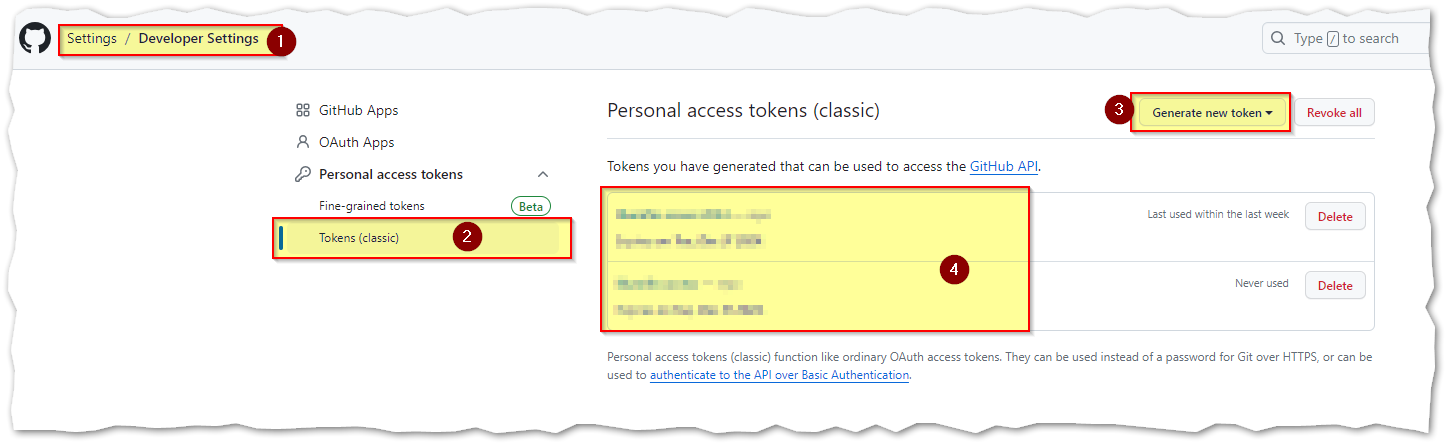
\includegraphics[width=200px]{images/Personal-Access-Tokens.png}
git config credential.helper 'store [<options>]'
\end{document}
